%%%%%%%%%%%%%%%%%%%%%%%%%%EJERCICIO 6a %%%%%%%%%%%%%%%%%%%%%%%%%%%
	
	\textbf{Ejemplo 6}\\
	Hallar la distribución del pago 58 en una amortización de 5.000.000 COP en pagos mensuales durante 10 años. Suponga que los pagos son crecientes en un 2\% y que la tasa es del 3\% periódico mes vencido.
	
	%\newpage %USAR SOLO SI EL SOLUCIÓN QUEDA SOLO Y ES NECESARIO BAJARLO A LA SIGUIENTE PAGINA
	
	\textbf{Solución 6.}\\
	%La tabla ira centrada
	\begin{center}
		\renewcommand{\arraystretch}{1.5}% Margenes de las celdas
		%Creación de la cuadricula de 3 columnas
		\begin{longtable}[H]{|p{0.5\linewidth}|p{0.5\linewidth}|}
			%Creamos una linea horizontal
			\hline
			%Definimos el color de la primera fila
			\rowcolor[HTML]{FFB183}
			%%%%% INICIO ASIGNACIÓN PERIODO FOCAL %%%%%%%
			%%%%%%%%%% INICIO TITULO
			%Lo que se hace aquí es mezclar las 3 columnas en una sola
			\multicolumn{2}{|c|}{\cellcolor[HTML]{FFB183}\textbf{1. Asignación período focal}}   \\ \hline
			%%%%%%%%%% FIN TITULO
			%%%%% INICIO DECLARACIÓN DE VARIABLES %%%%%%%
			\multicolumn{2}{|c|}{$pf = 0 \textit{ pmv}$}\\ \hline
			%%%%%%%%%% INICIO TITULO
			%Lo que se hace aquí es mezclar las 3 columnas en una sola
			\multicolumn{2}{|c|}{\cellcolor[HTML]{FFB183}\textbf{2. Declaración de variables}}   \\ \hline
			%%%%%%%%%% FIN TITULO
			%%%%%%%%%% INICIO DE MATEMÁTICAS
			%Cada & hace referencia al paso de la siguiente columna
			$VP = 5$.$000$.$000 \hspace{1mm} COP$  				& $n =120 \hspace{1mm} pmv $  \\
			$g = 2\% $      	                         & $R_{1}= ? \hspace{1mm} COP    $ \\
			$i  \equiv  3\%  \hspace{1mm} pmv$             & $ $ \\ \hline
			%%%%%%%%%% FIN DE MATEMÁTICAS
			%%%%% FIN DECLARACIÓN DE VARIABLES
			
			\rowcolor[HTML]{FFB183}
			\multicolumn{2}{|c|}{\cellcolor[HTML]{FFB183}\textbf{3. Diagrama de flujo de caja}} \\ \hline
			\multicolumn{2}{|c|}{ \includegraphics[trim=-78 -5 -78 -5]{7_Capitulo/img/ejemplos/6/6_1.pdf} }   \\ \hline
			%%%%% INICIO FLUJO DE CAJA
			\rowcolor[HTML]{FFB183}
			\multicolumn{2}{|c|}{\cellcolor[HTML]{FFB183}\textbf{4. Declaración de fórmulas}} \\ \hline
			%%%%%%%%%%%%% FIN INSERCIÓN DE IMAGEN
			%%%%%FIN FLUJO DE CAJA
			
			\multicolumn{2}{|c|}{ $VP = \frac{R(1+g)^{n} (1+i)^{n}-1}{g-i} $ Valor presente de un gradiente geométrico si g$ \vee $i }   \\ 
			\multicolumn{2}{|c|}{ $I = P \hspace{1mm} i $ Interés periódico }   \\ 
			\multicolumn{2}{|c|}{ $A = R - I $ Amortización a capital, una vez descontados los intereses de la cuota R }   \\ 
			\multicolumn{2}{|c|}{ $R_{n} = R_{1}(1 + g)^{n-1} $ Valor flujo de un gradiente aritmético }   \\ \hline
			
			%%%%%% INICIO DESARROLLO MATEMÁTICO
			\rowcolor[HTML]{FFB183}
			%%%%%%%%%%INICIO TITULO
			\multicolumn{2}{|c|}{\cellcolor[HTML]{FFB183}\textbf{5. Desarrollo matemático}}       \\ \hline
			%%%%%%%%%% FIN TITULO
			%%%%%%%%%% INICIO MATEMÁTICAS
			\multicolumn{2}{|C{\linewidth}|}{
				Lo primero es calcular R1 con el fin de poder hallar el valor de R58 y saber qué es lo que va a repartir.
				
				
				 $  5$.$000$.$000 \hspace{1mm} COP  = \frac{ R(1+ 0,02)^{120} (1+ 0,03)^{120}-1}{0,02- 0,03} $
				
				$R_{1} =  72$.$478,16 \hspace{1mm} COP$
				
				
			}\\ \hline
			
			%%%%%%%%%% FIN MATEMÁTICAS
			%%%%%% FIN DESARROLLO MATEMÁTICO
			%%%%%% INICIO RESPUESTA
			\rowcolor[HTML]{FFB183}
			%%%%%%%%%%INICIO TITULO
			\multicolumn{2}{|c|}{\cellcolor[HTML]{FFB183}\textbf{6. Respuesta}}   \\ \hline
			%%%%%%%%%% FIN TITULO
			%%%%%%%%%% INICIO RESPUESTA MATEMÁTICA
			%\multicolumn{2}{|c|}{ \includegraphics[trim=-78 -5 -78 -5]{7_Capitulo/img/ejemplos/5/5_2.jpg} }   \\ \hline
			\multicolumn{2}{|C{\textwidth}|}{
				$R_{58} =  72$.$478,16 \hspace{1mm} COP(1 + 0,02)^{57} =  224$.$087,15 \hspace{1mm} COP$ 
			}  \\ \hline
			
			
			%%%%%%%%%% FIN MATEMÁTICAS
			%%%%%% FIN RESPUESTA
		\end{longtable}
		%Se crean dos lineas en blanco para que no quede el siguiente texto tan pegado
		%\newline \newline %USARLO SI CREES QUE ES NECESARIO
	\end{center}
    %%%%%%%%%%%%%%%%%%%%%%%%%%FIN EJERCICIO 6a %%%%%%%%%%%%%%%%%%%%%%%%%%%